% Copyright 2004 by Till Tantau <tantau@users.sourceforge.net>.
%
% In principle, this file can be redistributed and/or modified under
% the terms of the GNU Public License, version 2.
%
% However, this file is supposed to be a template to be modified
% for your own needs. For this reason, if you use this file as a
% template and not specifically distribute it as part of a another
% package/program, I grant the extra permission to freely copy and
% modify this file as you see fit and even to delete this copyright
% notice. 

\documentclass{beamer}

\usepackage[utf8]{inputenc}
\usepackage[T1]{fontenc}
\usepackage[french]{babel}
\usepackage{soul}
\usepackage[lofdepth,lotdepth]{subfig}

% There are many different themes available for Beamer. A comprehensive
% list with examples is given here:
% http://deic.uab.es/~iblanes/beamer_gallery/index_by_theme.html
% You can uncomment the themes below if you would like to use a different
% one:
%\usetheme{AnnArbor}
%\usetheme{Antibes}
%\usetheme{Bergen}
\usetheme{Berkeley}
%\usetheme{Berlin}
%\usetheme{Boadilla}
%\usetheme{boxes}
%\usetheme{CambridgeUS}
%\usetheme{Copenhagen}
%\usetheme{Darmstadt}
%\usetheme{default}
%\usetheme{Frankfurt}
%\usetheme{Goettingen}
%\usetheme{Hannover}
%\usetheme{Ilmenau}
%\usetheme{JuanLesPins}
%\usetheme{Luebeck}
%\usetheme{Madrid}
%\usetheme{Malmoe}
%\usetheme{Marburg}
%\usetheme{Montpellier}
%\usetheme{PaloAlto}
%\usetheme{Pittsburgh}
%\usetheme{Rochester}
%\usetheme{Singapore}
%\usetheme{Szeged}
%\usetheme{Warsaw}

\title{Orbox}

% A subtitle is optional and this may be deleted
\subtitle{Soutenance de PFE}

\author{Pierre Robillard\inst{1} \and Frédéric Rayar\inst{2}}
% - Give the names in the same order as the appear in the paper.
% - Use the \inst{?} command only if the authors have different
%   affiliation.

\institute[Universities of Somewhere and Elsewhere] % (optional, but mostly needed)
{
  \inst{1}%
  Réalisation\\
  Étudiants DII 5A
  \and
  \inst{2}%
  Encadrant du projet\\
  PhD Candidate}
% - Use the \inst command only if there are several affiliations.
% - Keep it simple, no one is interested in your street address.

\date{Polytech Tours, \today}
% - Either use conference name or its abbreviation.
% - Not really informative to the audience, more for people (including
%   yourself) who are reading the slides online

\subject{Theoretical Computer Science}
% This is only inserted into the PDF information catalog. Can be left
% out. 

% If you have a file called "university-logo-filename.xxx", where xxx
% is a graphic format that can be processed by latex or pdflatex,
% resp., then you can add a logo as follows:

% \pgfdeclareimage[height=0.5cm]{university-logo}{university-logo-filename}
% \logo{\pgfuseimage{university-logo}}

% Delete this, if you do not want the table of contents to pop up at
% the beginning of each subsection:
% \AtBeginSubsection[]
% {
%   \begin{frame}<beamer>{Outline}
%     \tableofcontents[currentsection,currentsubsection]
%   \end{frame}
% }

% Let's get started
\begin{document}

\begin{frame}
  \titlepage
\end{frame}

\begin{frame}{Sommaire}
  \tableofcontents
  % You might wish to add the option [pausesections]
\end{frame}

% Section and subsections will appear in the presentation overview
% and table of contents.
\section{Introduction}

\subsection{Le concept}

\begin{frame}{Qu'est que la Orbox ?}

\begin{center}
    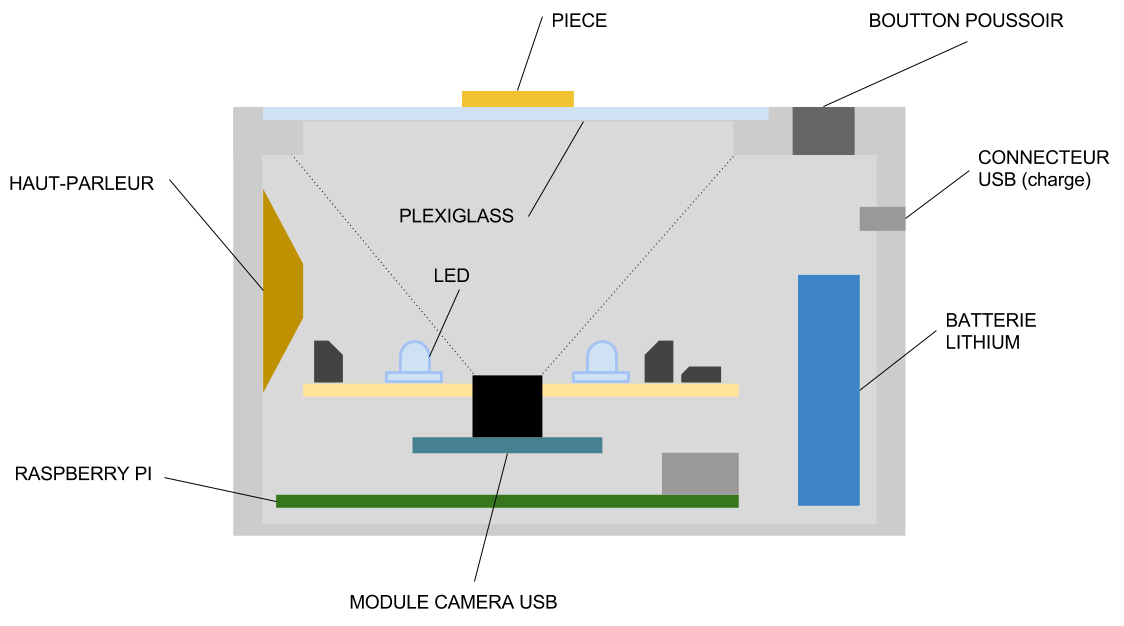
\includegraphics[width=7cm]{InitialSketch}
\end{center}

\begin{itemize}
    \item Un système destiné aux personnes souffrant de déficience visuelle.
    \item Délivrer à l’utilisateur des messages sonores sur les objets posé.

\end{itemize}

% \begin{block}{Block Title}
% You can also highlight sections of your presentation in a block, with it's own title
% \end{block}
% \begin{theorem}
% There are separate environments for theorems, examples, definitions and proofs.
% \end{theorem}
% \begin{example}
% Here is an example of an example block.
% \end{example}
\end{frame}

\subsection{Le contexte}

\begin{frame}{Les origines du projet}
Suite d'un projet collectif de quatrième année.\\
Sujet proposé et encadré par F. Rayar.

\begin{block}{Cons}
\begin{itemize}
    \item Taux de reconnaissance faible (~70\%)
    \item Pas d'intégration finale (pas de circuit imprimé)
\end{itemize}
\end{block}
\begin{block}{Pros}
\begin{itemize}
    \item Travail sur l'optique en place
    \item Pré-traitement de l'image effectué
\end{itemize}
\end{block}

\end{frame}

\subsection{Les objectifs}
\begin{frame}{Les objectifs du projet}
Il a été convenu avec la MOA des objectifs suivants :
\begin{itemize}
    \item Un \alert{prototype fonctionnel}.
    \item Les contraintes d'industrialisation ne seront \alert{pas} abordées.
    \item Un taux de reconnaissance de \alert{90\% minimum} sur le cas d'utilisation des pièces de monnaie d'euros.
\end{itemize}
\end{frame}

\section{Gestion de projet}
\subsection{Plannings}
\begin{frame}{Le planning prévisionnel}
\begin{center}
    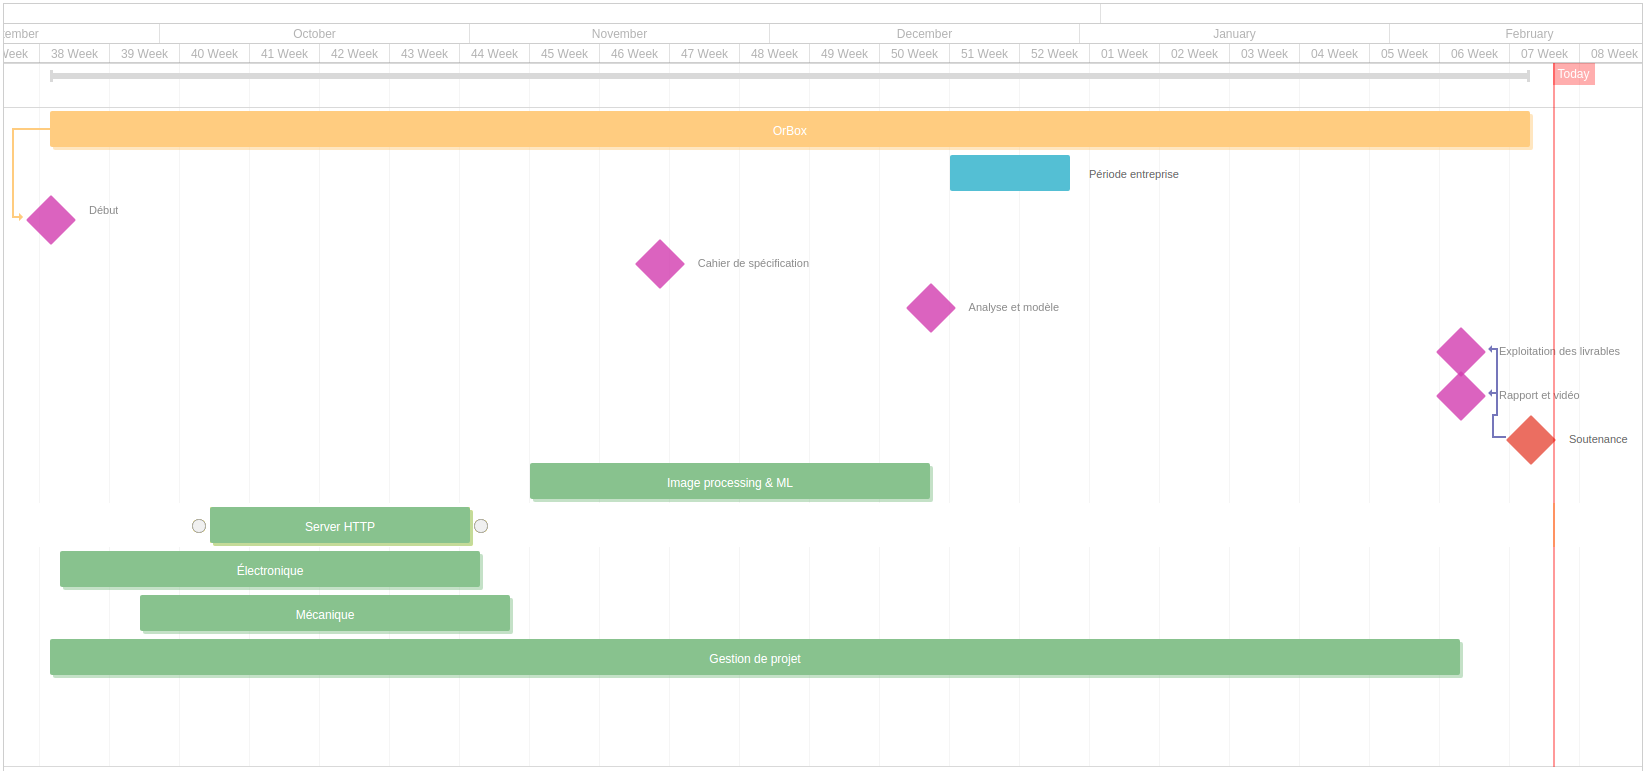
\includegraphics[width=11cm]{ganttproInit}
\end{center}
\end{frame}
\begin{frame}{Planning réel et écarts constatés}
\begin{center}
    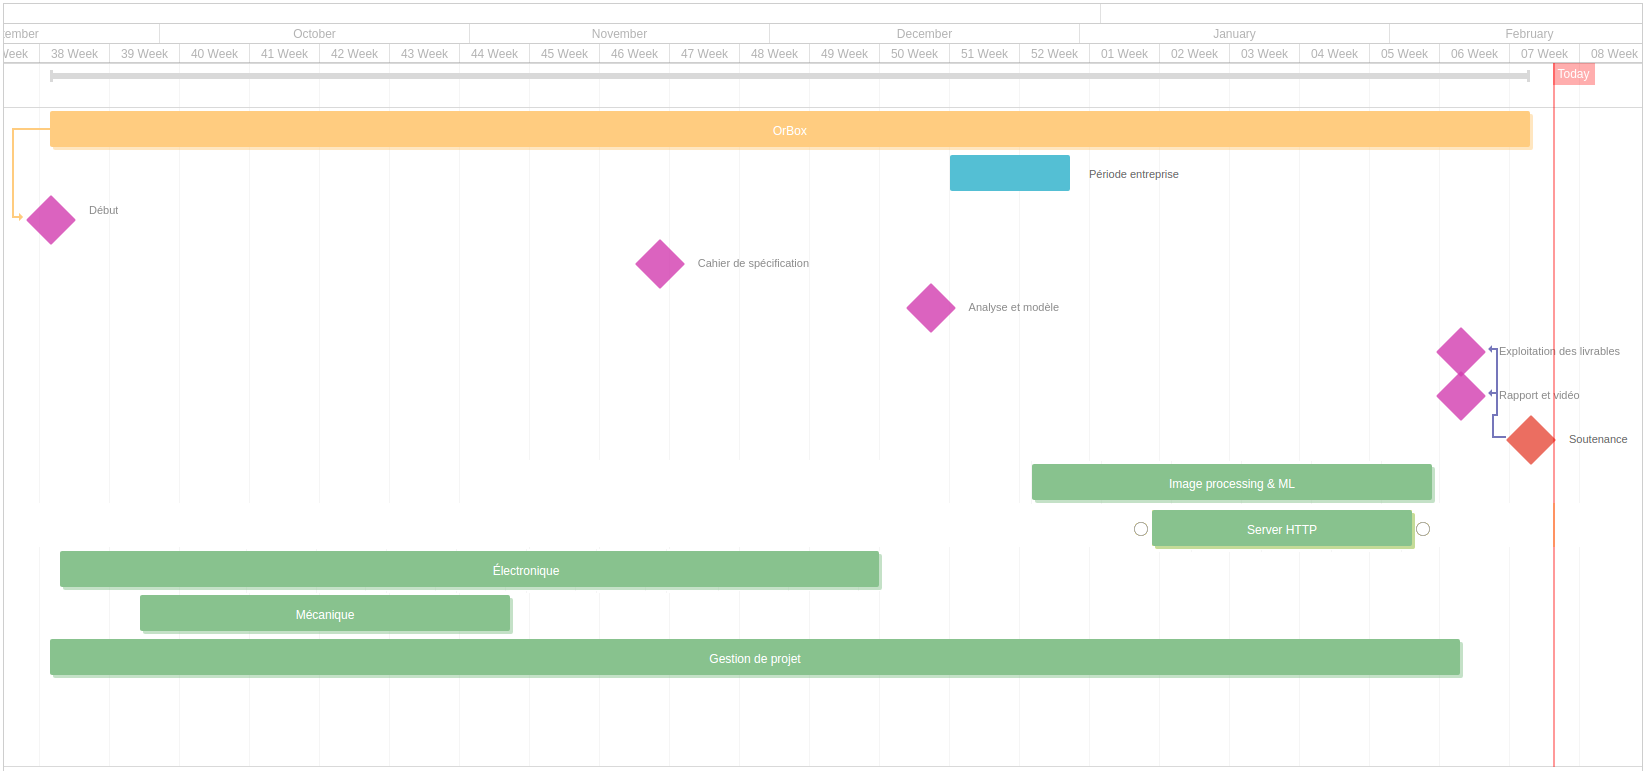
\includegraphics[width=11cm]{ganttproFinal}
\end{center}
\end{frame}

\section{Architecture}
\subsection{Modélisation}
\begin{frame}{Modélisation SysML du système}
  \begin{center}
    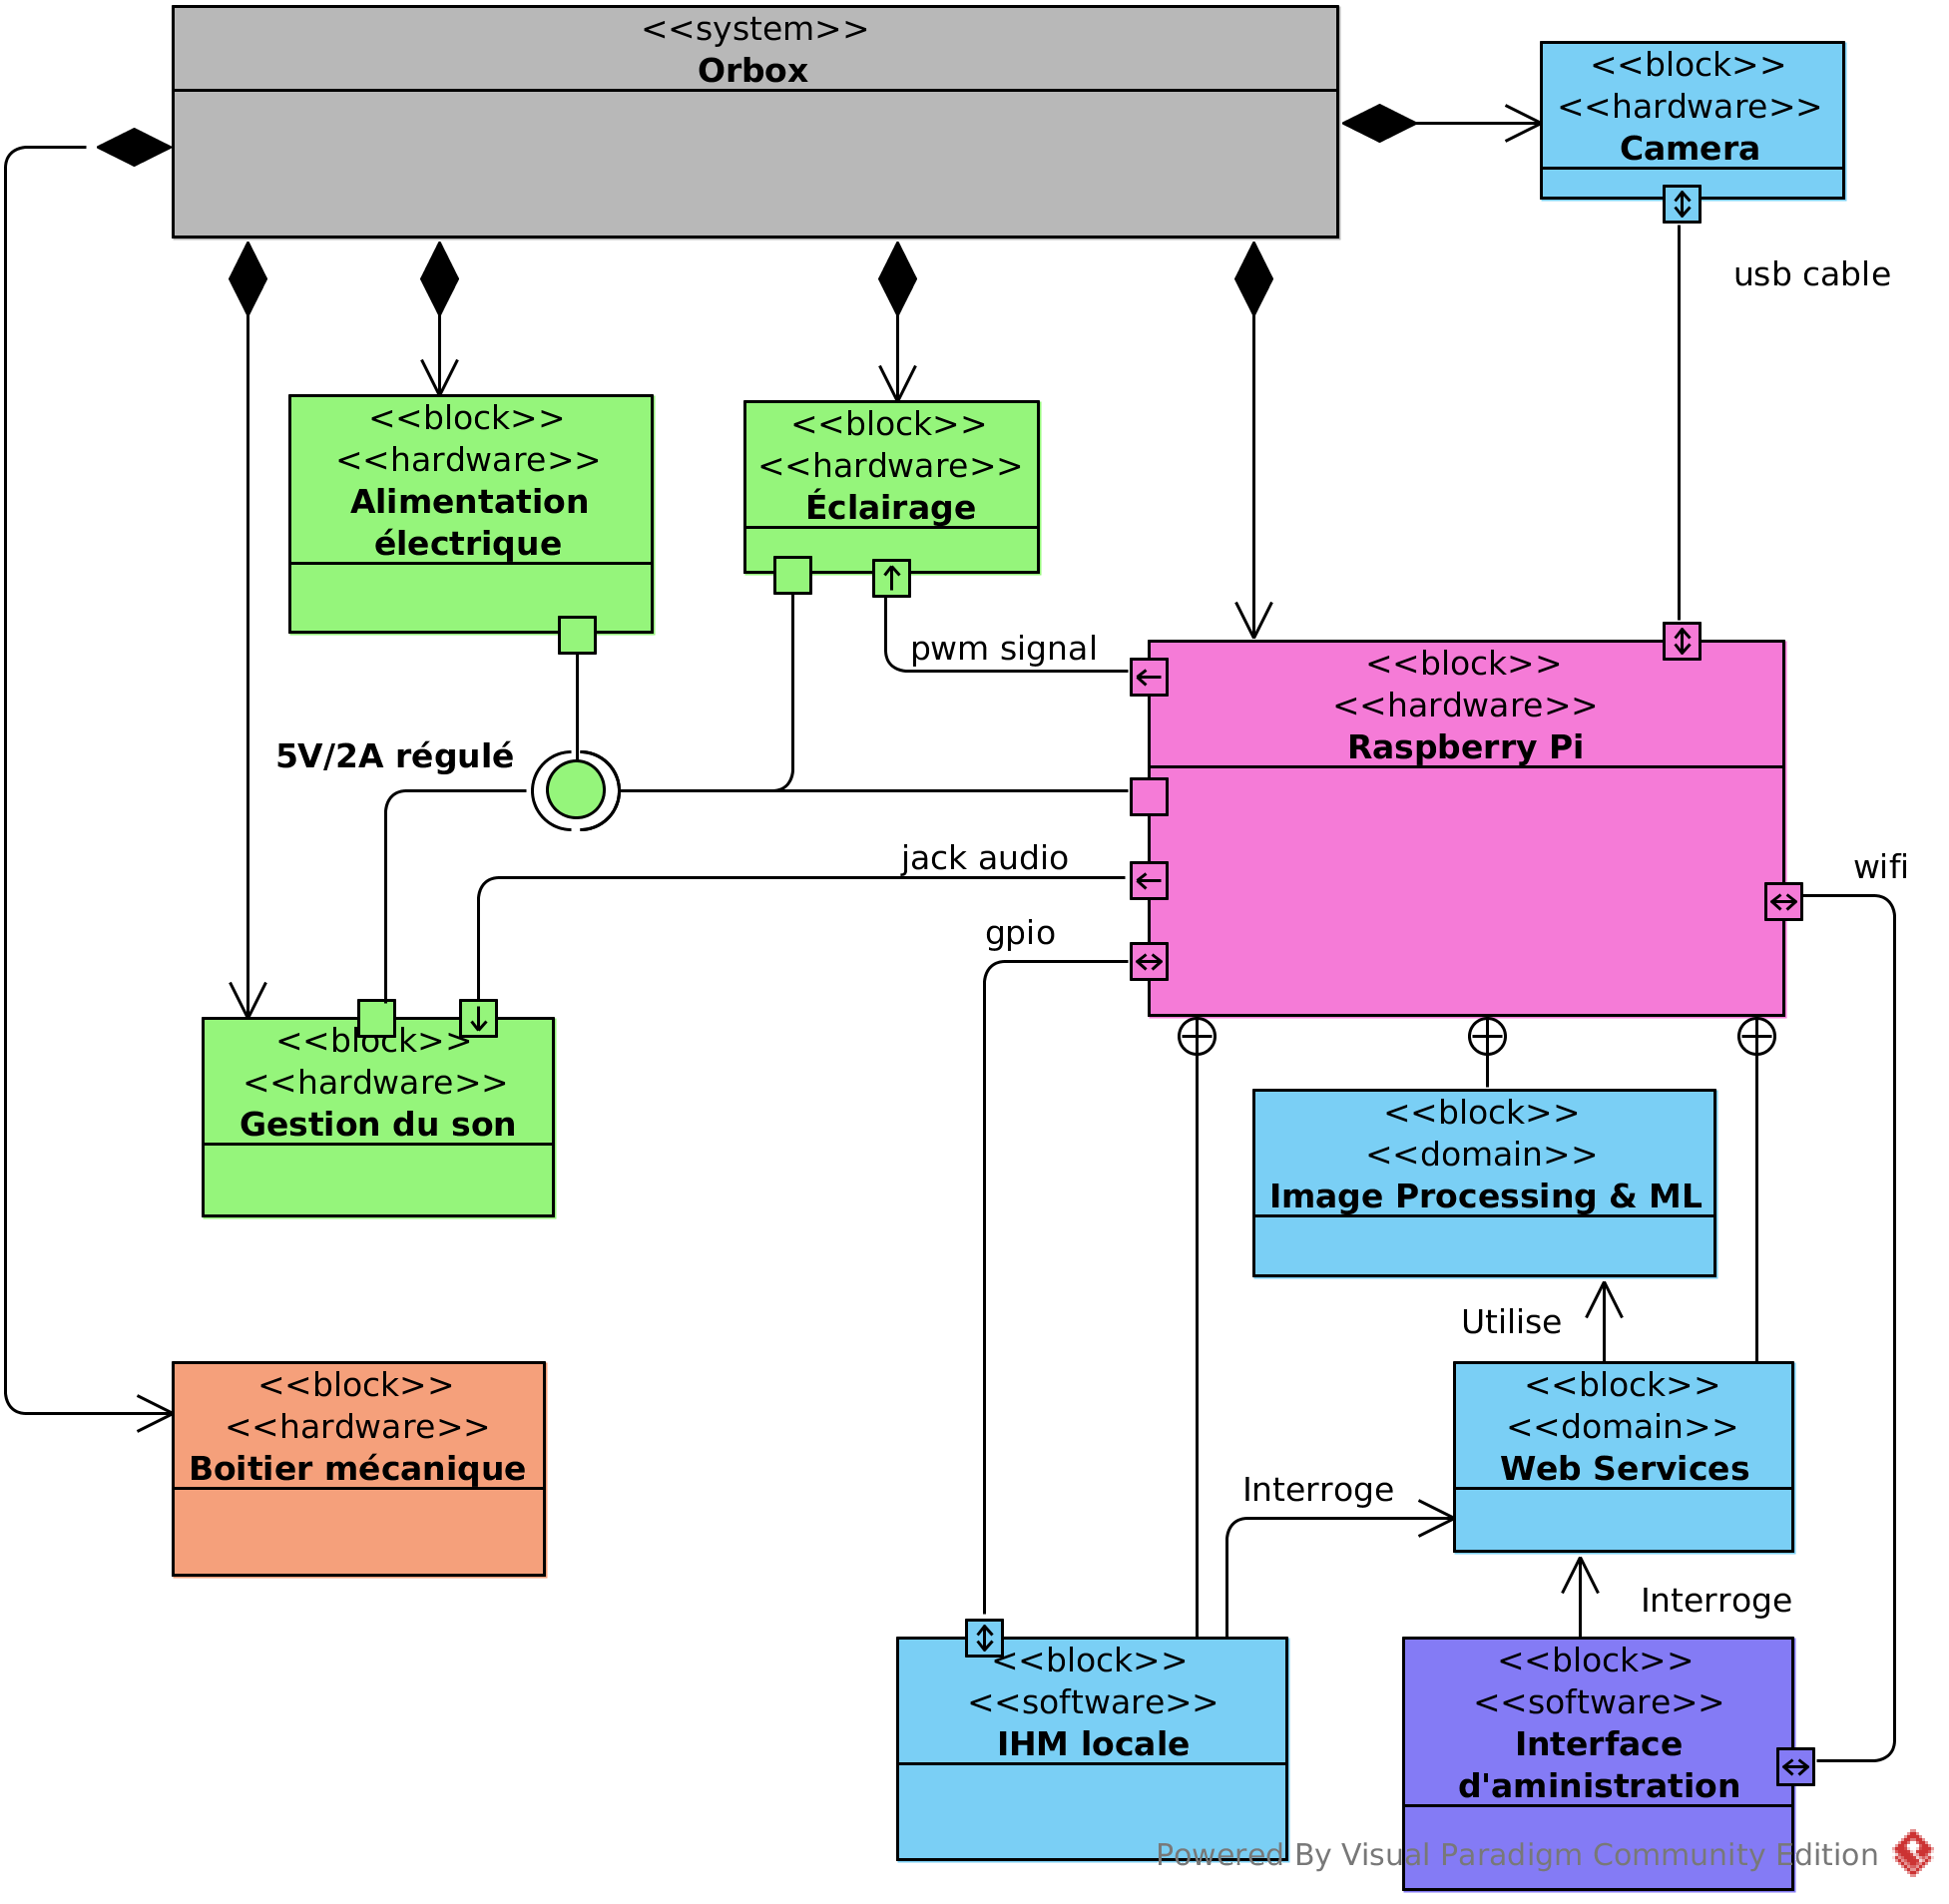
\includegraphics[width=7cm]{SysML_Top_BDD}
\end{center}
\end{frame}
\subsection{Concecption matérielle}
\begin{frame}{La conception hardware}
 \begin{itemize}
     \item L'électronique
     \begin{itemize}
         \item Retard $\sim$ 1 mois dans la fabrication du circuit imprimé.
         \item Problèmes d'accroche à l'allumage pour convertisseur DC/DC 3.7/5V
     \end{itemize}
     \item La mécanique
     \begin{itemize}
         \item Boitier réaliser sur \emph{OnShape}.
         \item Plexi et diffuseur $\mapsto$ existants.
     \end{itemize}
 \end{itemize}
 
 \begin{block}{}
Plus de reflet grâce au nouvel éclairage et boitier.\\
Pas besoin de traitement numérique.
\end{block}
  
\end{frame}

\section{Analyse logicielle}
\subsection{Interface d'administration}
\begin{frame}{L'interface d'administration}
Elle doit permettre l'enrichissement de la base de données.
\begin{itemize}
    \item \st{Mongo DB} $\rightarrow$ Sérialization en fichier JSON.
    \item \st{Scalatra} $\rightarrow$ NodeJS.
\end{itemize}

\begin{block}{}
Une démonstration !
\end{block}

\end{frame}
\subsection{Traitement d'image}
\begin{frame}{Pre-processing et ségmentation}

\begin{figure}[H]
    \centering
    \subfloat[Différence absolue]{
        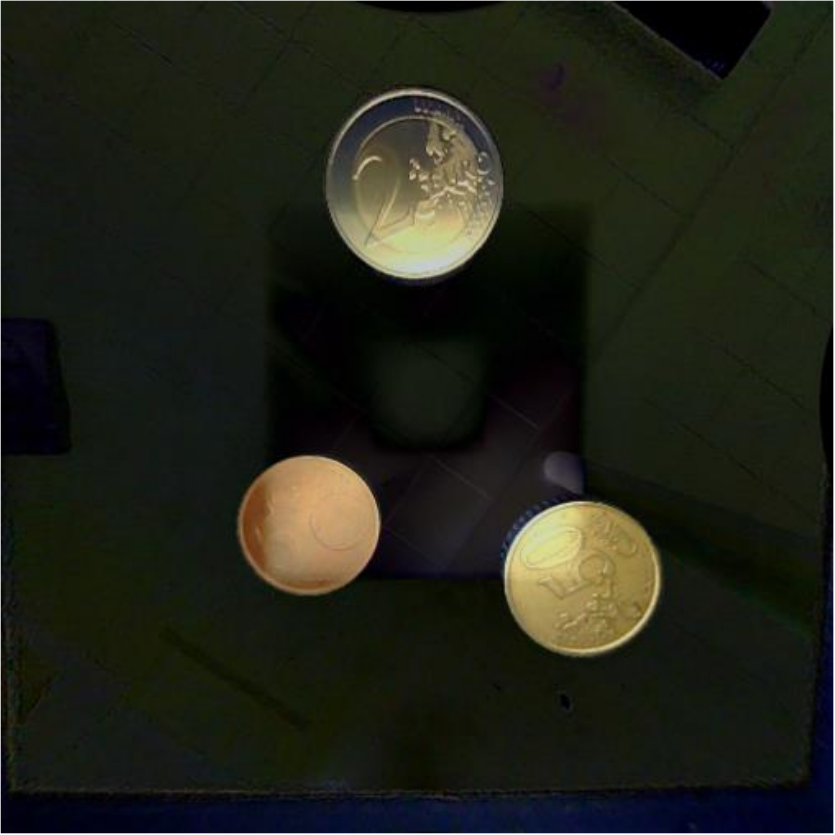
\includegraphics[width=0.25\textwidth]{Segmentation_AbsDiff}
        \label{Segmentation_AbsDiff}
    }
    \subfloat[Canal de teinte flouté]{
        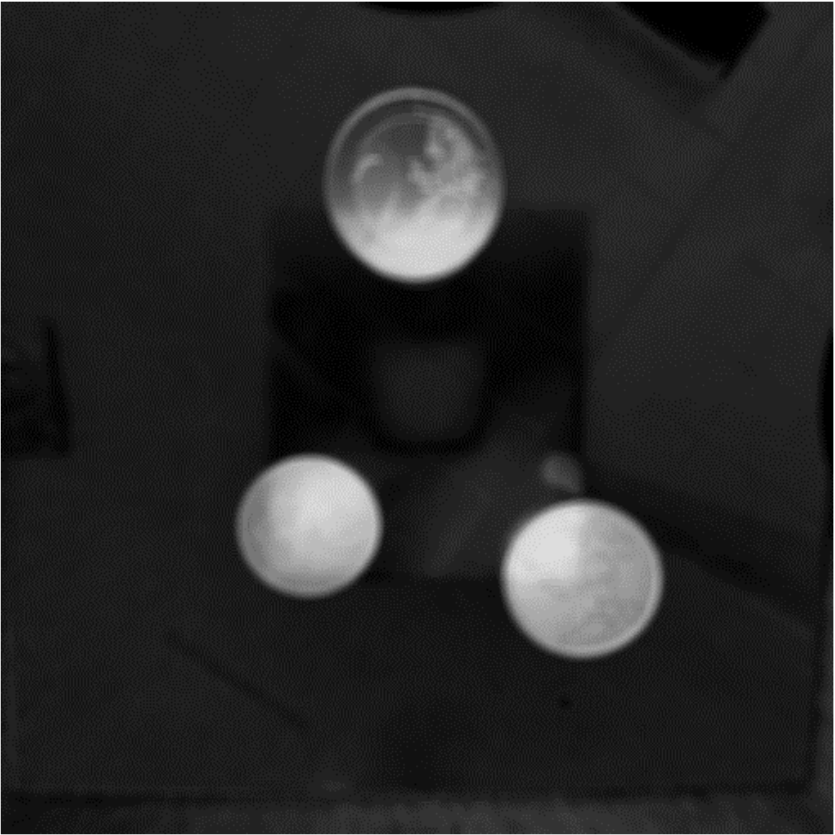
\includegraphics[width=0.25\textwidth]{Segmentation_HueBlurred}
        \label{Segmentation_HueBlurred}
    }
    \subfloat[Seuillage]{
        
\includegraphics[width=0.25\textwidth]{Segmentation_Threshold}
        \label{Segmentation_Threshold}
    }
    \qquad
    \subfloat[Érosion]{
        
\includegraphics[width=0.25\textwidth]{Segmentation_Erosion}
        \label{Segmentation_Erosion}
    }
    \subfloat[Dilatation]{
        
\includegraphics[width=0.25\textwidth]{Segmentation_Dilatation}
        \label{Segmentation_Dilatation}
    }
    \subfloat[Rectangles circonscrit]{
        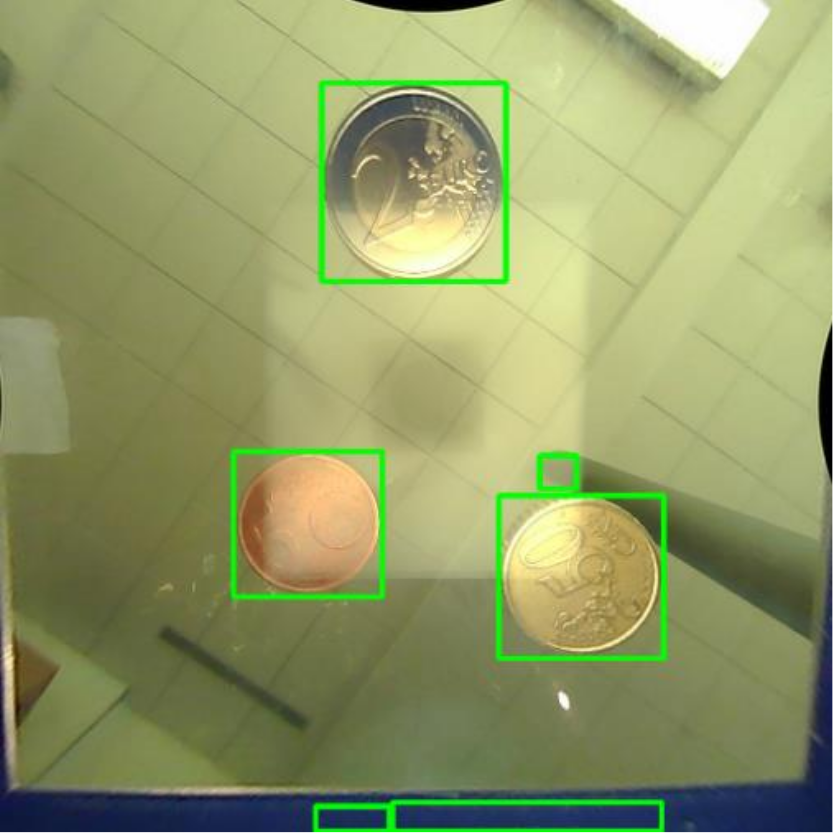
\includegraphics[width=0.25\textwidth]{Segmentation_BoundRect}
        \label{Segmentation_BoundRect}
    }
    \caption{Processus de segmentation}
    \label{segfig}
\end{figure}
  
\end{frame}
\subsection{Classificateur}
\begin{frame}{Les descripteurs utilisés}
Shape-based/contour-based descriptors :
\begin{itemize}
\item Le périmètre
\item L'aire
\item La circularité
\item Largeur/Hauteur du rectangle circonscrit d'aire minimum
\end{itemize}
            
Color-based descriptors.
\begin{itemize}
\item Histogramme de teinte normalisé.
\end{itemize}

\end{frame}
\begin{frame}{Protocole d'évaluation expérimentale}

\begin{itemize}
    \item Validation croisé en \emph{"k-fold cross validation"}.
    \item Chaque échantillon est utilisé exactement une fois comme ensemble de validation.
\end{itemize}


\begin{center}
    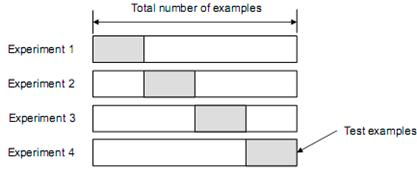
\includegraphics[width=6cm]{image002}
\end{center}
  
\end{frame}
\begin{frame}{Résultats}
 \begin{table}[]
\centering
\begin{tabular}{lll}
\textbf{Descripteurs utilisés}                                                   & \textbf{Classificateur} & \textbf{Erreur moyenne} \\ \hline
Aire et 60 barres d'hist.                                               & 1-NN           & 20.17\%                 \\ \hline
Aire et 60 barres d'hist.                                                & 9-NN           & 22.14 \%                \\ \hline
Tous \& 15/42 b. d'hist. & SVM RBF         & 12.61\%                 \\ \hline
Tous \& 15/42 b. d'hist. & SVM Sigmoïd     & 78.23\%                 \\ \hline
Tous \& 15/42 b. d'hist. & SVM CHI2       & 7.42\%                 
\end{tabular}
\end{table}

Les KNN sont testés en 150-fold cross validation.
Les SVM sont testés en 20-fold cross validation.
\end{frame}

% Placing a * after \section means it will not show in the
% outline or table of contents.
\section*{Conclusion}

\begin{frame}{Conclusion}

Les objectifs du PFE ont été atteints :
\begin{itemize}
    \item Fabrication d'un \alert{prototype fonctionnel}.
    \item Erreur de \alert{moins de 10 \%} sur le cas d'utilisation des pièces de monnaie d'euros.
\end{itemize}
Cependant, pas de temps pour :
\begin{itemize}
    \item Une autre base d'apprentissage.
    \item D'autre descripteurs/classificateurs.
\end{itemize}
\end{frame}



% All of the following is optional and typically not needed. 
% \appendix
% \section<presentation>*{\appendixname}
% \subsection<presentation>*{For Further Reading}

% \begin{frame}[allowframebreaks]
%   \frametitle<presentation>{For Further Reading}
    
%   \begin{thebibliography}{10}
    
%   \beamertemplatebookbibitems
%   % Start with overview books.

%   \bibitem{Author1990}
%     A.~Author.
%     \newblock {\em Handbook of Everything}.
%     \newblock Some Press, 1990.
 
    
%   \beamertemplatearticlebibitems
%   % Followed by interesting articles. Keep the list short. 

%   \bibitem{Someone2000}
%     S.~Someone.
%     \newblock On this and that.
%     \newblock {\em Journal of This and That}, 2(1):50--100,
%     2000.
%   \end{thebibliography}
% \end{frame}

\end{document}


